\documentclass[t, serif, 8 pt]{beamer}
\usepackage[utf8]{inputenc}
\usepackage{graphicx}
\usepackage{xcolor}
\usepackage{subfigure}
\usepackage[absolute,overlay]{textpos}
\usepackage{tikz-feynman}
%\usepackage{comment}
\usepackage{hyperref}
\usepackage{pdfpages}
\usepackage{pifont}
\usepackage{textcomp}
%%\hypersetup{colorlinks=true}
\usepackage{tikz}
\usepackage{multirow}
\usepackage{ amssymb }
\setlength{\unitlength}{1 cm} 
%L%\definecolor{blue}{rgb}{0.8,0.8,1.0}
\usepackage{appendix}
\usepackage{palatino}
\usepackage{verbatim}
\usepackage{slashed}
\usepackage{xspace}
\usepackage{xcolor,colortbl}
%\usepackage{arydshln}
\usepackage[export]{adjustbox}

%non contare le slides in backup
%\usepackage{appendixnumberbeamer}
%\newcommand{\backupbegin}{
%   \newcounter{finalframe}
%   \setcounter{finalframe}{\value{framenumber}}
%}
%\newcommand{\backupend}{
%   \setcounter{framenumber}{\value{finalframe}}
%}

%Mai provato questo
%\newtheorem{examplefirst}{Example}
%\newenvironment<>{examplefirst}[1][]{%
%  \setbeamercolor{block title example}{fg=white,bg=red!75!black}%
%  \begin{example}#2[#1]}{\end{example}}

%Environment block
\newenvironment<>{variableblock}[3]{%
  \setbeamercolor{block body}{#2}
  \setbeamercolor{block title}{#3}
  \begin{block}{#1}}{\end{block}}

\newenvironment<>{lisablock}[2]{%
  \setbeamercolor{block body}{#2}
  \begin{block}{#1}}{\end{block}}

\usetheme{Szeged}%Ilmenau
% PaloAlto
% JuanLesPins e' orribile ma almeno si legge tutto
% Szeged non si leggono le sections
\usecolortheme{beaver}
% beaver, seahorse
\usepackage[english]{babel}
%\usepackage[latin1]{inputenc}
\setbeamercovered{transparent}

\usepackage[math]{iwona}
\usepackage[T1]{fontenc}

%modifico forma ITEM
\setbeamertemplate{itemize items}[circle]
%\newcommand{\myitem}{\item[$\hookrightarrow$]}
\newcommand{\staritem}{\item[\ding{71}]}
\newcommand{\myitem}{\item[\ding{224}]}
\newcommand{\cmark}{\ding{51}}%
\newcommand{\xmark}{\ding{55}}%

\newcommand{\VZ}{\ensuremath{VZ}\xspace}
\newcommand{\met}{\ensuremath{\vec{p}_T^{\text{miss}}}\xspace}
\newcommand{\MET}{\ensuremath{E_T^{\text{miss}}}\xspace}
\newcommand{\mtVZ}{\ensuremath{m_{\VZ}^T}\xspace}
\newcommand{\mVZ}{\ensuremath{m_{\VZ}}\xspace}

%IMPORTANTE: PER TENERE TITOLO E ANCHE NUMERO DI PAGINA!!!
    \expandafter\def\expandafter\insertshorttitle\expandafter{%
      \insertshorttitle\hfill%
      \insertframenumber\,/\,\inserttotalframenumber}
%\setbeamertemplate{footline}[frame number]
%\title{{\bf Search for heavy lepton partners of neutrinos in 2012 CMS data}}
%\subtitle{\bf{in the context of type III seesaw mechanism}}

%%%% ESEMPIO COLONNE
%\begin{frame}
%\frametitle{Incosistency}
%\begin{columns}[c]
%    \column{.5\textwidth}
%        \begin{center}
%            \includegraphics[scale=0.3]{peer}
%        \end{center}
%    \column{.5\texwidth}
%        \begin{center}
%             \includegraphics[scale=0.3]{peer-inconsistent} 
%        \end{center}
%\end{columns}
%\end{frame}

\title{{\bf Search for heavy resonances decaying into a $Z$ boson and a vector boson in the $\nu \bar{\nu}$ $q\bar{q}$ final state at CMS}}
%\subtitle{\bf Approval}
\date{}
\addtobeamertemplate{footline}{}{%
\begin{tikzpicture}[remember picture,overlay]
\pgfdeclareimage[height=0.06\paperwidth]{logo}{../cms}
\node at (current page.south east) [xshift=-0.03\paperwidth,yshift=0.673\paperwidth,opacity=1] (flogo) {\pgfuseimage{logo}};
\end{tikzpicture}
\begin{tikzpicture}[remember picture,overlay]
\pgfdeclareimage[height=0.06\paperwidth]{logo}{../logo2}%{logo_unipd2_piccolo}
\node at (current page.south east) [xshift=-0.094\paperwidth,yshift=0.673\paperwidth,opacity=1] (flogo) {\pgfuseimage{logo}};
\end{tikzpicture}
%\begin{tikzpicture}[remember picture,overlay]
%\pgfdeclareimage[height=0.06\paperwidth]{logo}{../university-of-zurich-logo}
%\node at (current page.south east) [xshift=-0.155\paperwidth,yshift=0.673\paperwidth,opacity=1] (flogo) {\pgfuseimage{logo}};
%\end{tikzpicture}
%\begin{tikzpicture}[remember picture,overlay]
%\pgfdeclareimage[height=0.06\paperwidth]{logo}{../BROWN-UNIVERSITY-SEAL}
%\node at (current page.south east) [xshift=-0.205\paperwidth,yshift=0.673\paperwidth,opacity=1] (flogo) {\pgfuseimage{logo}};
%\end{tikzpicture}
\begin{tikzpicture}[remember picture,overlay]
\pgfdeclareimage[height=0.06\paperwidth]{logo}{../weblogo1b}
\node at (current page.south east) [xshift=-0.155\paperwidth,yshift=0.673\paperwidth,opacity=1] (flogo) {\pgfuseimage{logo}};
\end{tikzpicture}
}

\begin{document}
\renewcommand{\inserttotalframenumber}{33}

\begin{frame}
\maketitle
\vspace*{-2cm}
\begin{center}
%\includegraphics[width=3cm]{../eventdisplay.png}
\includegraphics[width=2.cm]{../logo2}
\end{center}
\begin{variableblock}{\center \small{Corso di Dottorato di Ricerca in Fisica \\ XXX ciclo \\ \vspace*{1\baselineskip} Padova, 26 marzo 2018}}{bg=gray!5,fg=black}{bg=gray!10,fg=red!80!black}
\vspace*{-0.3cm}
\center{\small{ \textbf{Coordinatore:} Ch.mo Prof. Gianguido Dall'Agata \\ \textbf{Supervisore}: Ch.mo Prof. Franco Simonetto \\ \vspace*{1\baselineskip} \textbf{Dottoranda}: Lisa Benato}}
\end{variableblock}
\end{frame}


%
%column copypaste
%\begin{columns}
%\begin{column}{0.5\textwidth}
%\begin{variableblock}{\small Text block}{bg=gray!5,fg=black}{bg=gray!10,fg=red!80!black}
%\end{variableblock}
%\end{column}
%\begin{column}{0.5\textwidth}
%\begin{variableblock}{\small Text block}{bg=gray!5,fg=black}{bg=gray!10,fg=red!80!black}
%\end{variableblock}
%\end{column}
%\end{columns}

\begin{frame}
\frametitle{Outline}
\begin{columns}
\begin{column}{0.5\textwidth}

\begin{lisablock}{}{bg=blue!10,fg=black}
\centering
1. Motivations
\end{lisablock}

\vspace*{0.5cm}

\begin{lisablock}{}{bg=red!10,fg=black}
\centering
2. Signal signatures of the models probed
\end{lisablock}

\vspace*{0.5cm}

\begin{lisablock}{}{bg=green!10,fg=black}
\centering
3. Reconstructed physics objects and selections
\end{lisablock}

\end{column}
\begin{column}{0.5\textwidth}

\begin{lisablock}{}{bg=yellow!10,fg=black}
\centering
4. Background prediction
\end{lisablock}

\vspace*{0.5cm}

\begin{lisablock}{}{bg=gray!10,fg=black}
\centering
5. Results and interpretation
\end{lisablock}

\vspace*{0.5cm}

\begin{lisablock}{}{bg=cyan!10,fg=black}
\centering
6. Future perspectives and conclusion
\end{lisablock}

\end{column}
\end{columns}
\end{frame}


\begin{frame}
\frametitle{Motivations}
\small
\vspace*{-0.5cm}
\begin{columns}
\begin{column}{0.5\textwidth}
\begin{variableblock}{\small Standard Model of particles}{bg=gray!5,fg=black}{bg=gray!10,fg=red!80!black}
\begin{itemize}
\item Standard Model (SM): the best description of elementary particles and their interactions
\item Summation of electromagnetic, weak and strong interactions: $SU_C(3) \times SU_L(2) \times U_Y (1)$
\item Higgs scalar field gives mass to fermions and weak bosons via spontaneous symmetry breaking
\end{itemize}
%General problems of SM, nice picture, hierarchy problem: different scales are not decoupled, high energy scale corrects the higgs mass, fine tuning cancellation\\
\vspace*{-0.2cm}
\begin{center}
\includegraphics[width = 0.83 \textwidth]{SM.png}
\end{center}
\end{variableblock}
\end{column}

\begin{column}{0.5\textwidth}
\begin{variableblock}{\small SM open problems}{bg=gray!5,fg=black}{bg=gray!10,fg=red!80!black}
\begin{itemize}
\item[0.] phenomenological observations not included (neutrino masses, dark matter candidates, cosmological inflation, matter-antimatter asymmetry)
%\item theoretical issues
\item[1.] flavour problem (too many free parameters)
\item[2.] no complete unification ($\alpha_{\text{em}}$, $\alpha_{\text{weak}}$, $\alpha_{\text{strong}}$, gravitation excluded)
\item[3.] {\bf hierarchy problem}:
%\begin{itemize}
\myitem electroweak ($\sim 100$ GeV) and Planck ($\sim 10^{19}$ GeV) scales are not decoupled
\myitem Higgs mass is UV-sensitive: divergencies require fine tuning cancellations (1 over $10^{34}$)
%\end{itemize}
\end{itemize}

%One-loop corrections to the Higgs mass. The three diagrams are quadratically divergent and make the Higgs mass highly UV-sensitive.\\
\begin{center}
\includegraphics[width = 0.8 \textwidth]{loop_corrections.jpg}
\end{center}
\vspace*{-0.1cm}
\begin{itemize}
\item Solutions: enlarging the SM gauge group
\myitem Grand Unification Theories, SUper SYmmetry..
\end{itemize}
\end{variableblock}

\end{column}

\end{columns}
\end{frame}

\begin{frame}
\frametitle{Heavy Vector Triplet}
\small
\vspace*{-0.5cm}
\begin{columns}
\begin{column}{0.5\textwidth}
\begin{variableblock}{\small HVT in a nutshell}{bg=gray!5,fg=black}{bg=gray!10,fg=red!80!black}
\begin{itemize}
\small
\item General framework (including Little Higgs, Composite Higgs, Sequential Standard Model)
%\begin{itemize}
\myitem Introduction a triplet of spin-1 $(X^0,X^+,X^-)$ ($Z'$,$W'$)
\myitem Simplified model: effective Lagrangian $\rightarrow$ relevant on-shell physics quantities (cross-section, width, mass of the resonance)
\myitem Few additional parameters in the SM Lagrangian: $g_V$ (strength), $c_H$ (coupling to bosons), $c_F$ (coupling to fermions)
%\end{itemize}
\item HVT triplet protects the Higgs mass if $M_X \sim 1 $ TeV: $$m_{\text{W,Z}}/M_{\text{X}} \ll 1$$
\begin{itemize}
\myitem SM is reproduced within 1\% accuracy (small mixing of $X$ with weak fields)
\myitem no need of fine-tuning
\end{itemize}
\end{itemize}
\end{variableblock}
\end{column}

\begin{column}{0.5\textwidth}
\begin{variableblock}{\small $Z'$, $W'$ phenomenology and benchmark scenarios}{bg=gray!5,fg=black}{bg=gray!10,fg=red!80!black}
\begin{itemize}
\item HVT production and decays completely determined by $g_V$, $c_H$, $c_F$, $M_X$
\myitem $X$ produced mainly via $q \bar{q}$ scattering (Drell-Yan)
\myitem HVT-A model -- weak coupling: $BR(X \rightarrow f \bar{f})$ dominates (SSM-like)
\myitem HVT-B model -- strong coupling: $BR(X \rightarrow VV) \approx BR(X \rightarrow VH)$ dominates (Composite Higgs-like)%$\\$BR(X \rightarrow f \bar{f}) << BR(X \rightarrow VV) \approx BR(X \rightarrow VH)$
%\vspace*{-0.4cm}
	\begin{center}
%\includegraphics[width=0.4\textwidth]{hvt-zp-brs.pdf}
\includegraphics[width=0.8\textwidth]{hvt-wp-brs.pdf}
	\end{center}
\myitem HVT resonances are narrow (1\% of $m_X$)
\end{itemize}
\end{variableblock}
\end{column}
\end{columns}
\end{frame}

\begin{frame}
\frametitle{Warped extra dimensions}
\small
\vspace*{-0.5cm}
\begin{columns}
\begin{column}{0.5\textwidth}
\begin{variableblock}{\small Bulk WED in a nutshell}{bg=gray!5,fg=black}{bg=gray!10,fg=red!80!black}
\begin{itemize}
\small
\item Randall-Sundrum model:
%\begin{itemize}
\myitem 5th additional warped extra dimension% $\varphi$: 
$$ds^2 = e^{-2 k r_c \varphi} \eta_{\mu \nu} dx^{\mu} dx^{\nu} + r_c^2 d{\varphi}^2$$
\myitem spin-2 gravitons: modes $h_{\mu \nu}$ of the quantum fluctuations, expanded in Kaluza-Klein towers
\myitem TeV-brane and Planck-brane located at $\varphi=(\pi, 0)$
\myitem small $r_c$ generates large hierarchy between Planck--Higgs scales: $$m = e^{-k r_c \pi} m_0$$
%\end{itemize}
%\begin{itemize}
%\myitem Gravitons produced at TeV scale via gluon fusion, significant branching ratio into bosons
%\end{itemize}
\end{itemize}
\vspace*{-0.4cm}
\begin{center}
%\includegraphics[width=0.4\textwidth]{hvt-wp-brs.pdf}
\includegraphics[width=0.75\textwidth]{SUSY19c.png}
%\includegraphics[width=0.8\textwidth]{Brane.png}
\end{center}
\end{variableblock}
\end{column}

\begin{column}{0.5\textwidth}
\begin{variableblock}{\small Bulk gravitons phenomenology}{bg=gray!5,fg=black}{bg=gray!10,fg=red!80!black}

\begin{itemize}
\small
\item Bulk extension of the RS model:
%\begin{itemize}
\myitem Higgs sector $\leftrightarrow$ TeV brane; \\ light fermions $\rightarrow$ Planck brane;\\ heavy fermions $\rightarrow$ TeV brane
\myitem natural solution of the flavour problem %(Higgs coupling to heavy quarks)
\myitem small interaction of massive KK bulk gravitons $G$ with light fermions $\rightarrow$ $G$ produced via gluon fusion
\myitem significant branching ratio into bosons
%\end{itemize}
\item $G$ production and decays determined by
%\begin{itemize}
\myitem graviton mass $m_G$
\myitem curvature parameter $\tilde{k} = k / \bar{M_{Pl}}$;\\ if $\tilde{k}<1$ $\rightarrow$ $G$ narrow
%\end{itemize}
\end{itemize}
\vspace*{-0.4cm}
\begin{center}
%\includegraphics[width=0.4\textwidth]{hvt-wp-brs.pdf}
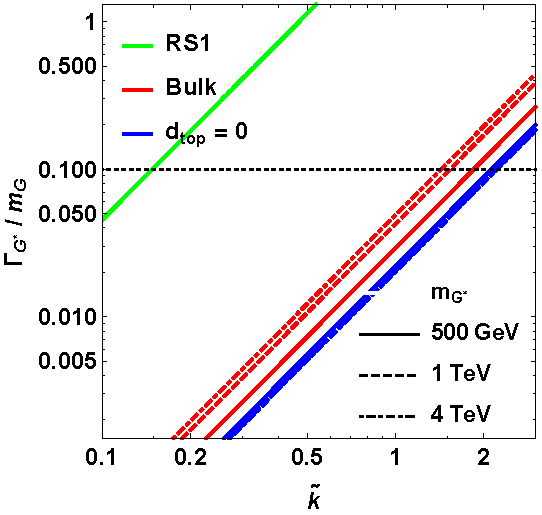
\includegraphics[width=0.45\textwidth]{../../figures/1404_0102_fig.pdf}
%\includegraphics[width=0.8\textwidth]{Brane.png}
\end{center}
\end{variableblock}
\end{column}
\end{columns}
\end{frame}

\begin{frame}
\frametitle{Data-driven motivation: previous results}
\vspace*{-0.5cm}
\small
\begin{columns}
\begin{column}{0.5\textwidth}
\begin{variableblock}{\color{red!80!black} \small Diboson excesses}{bg=gray!5,fg=black}{bg=gray!10,fg=red!80!black}
\small
CMS EXO-13-009, 2012 data: local excess @ 1.8 TeV (2. $\sigma$)
	\begin{center}
	\includegraphics[width=0.6\textwidth]{CMS_EXO_13_009.png}
	\end{center}
\small
ATLAS-CONF-2016-083, 2016 reduced dataset: local excess @ 1.6 TeV (2.5 $\sigma$), @ 3 TeV (3.5 $\sigma$)
	\begin{center}
	\includegraphics[width=0.6\textwidth]{ATL_previous.pdf}
	\end{center}
\end{variableblock}
\end{column}

\begin{column}{0.5\textwidth}
\begin{variableblock}{\color{red!80!black} \small The infamous $\gamma \gamma$ bump... was a diboson too!}{bg=gray!5,fg=black}{bg=gray!10,fg=red!80!black}
\small
CMS EXO-15-004, 2015 data: local excess @ 760 GeV (2.6 $\sigma$)
	\begin{center}
	\includegraphics[width=0.6\textwidth]{EXO-15-004-limits.png}

	\includegraphics[width=0.6\textwidth]{EXO-15-004-pvalue.pdf}
	\end{center}
\end{variableblock}
\vspace*{-0.3cm}
\begin{itemize}
\small
\item Rising interest in diboson resonances
\item Probing (almost) all the final states..
\end{itemize}

\end{column}
\end{columns}
\end{frame}


\begin{frame}
\frametitle{Machines for hunting heavy resonances}
\small
\vspace*{-0.5cm}
\begin{columns}
\begin{column}{0.4\textwidth}
\begin{variableblock}{\small LHC: producing heavy particles}{bg=gray!5,fg=black}{bg=gray!10,fg=red!80!black}

\begin{figure}[!htb]
\resizebox{.99\textwidth}{!}
{
  \centering
%\feynmandiagram [horizontal=a to b] {
%  i1 [particle=\(q\)] -- [fermion] a -- [fermion] i2 [particle=\(\overline{q} \)],
%  a -- [red!80!black, boson, edge label=\(V^{0}\), very thick] b,
%  f1 [particle=\(\overline{\ell}\)] -- [fermion] b -- [fermion] f2 [particle=\(\ell\)],
%};
%
\feynmandiagram [horizontal=a to b] {
  i1 [particle=\(q\)] -- [fermion] a -- [fermion] i2 [particle=\(\overline{q}'\)],
  a -- [red!80!black, boson, edge label=\(V^{-}\), very thick] b,
  f1 [particle=\(Z\)] -- [boson] b -- [boson] f2 [particle=\(W^{-}\)],
};

\feynmandiagram [horizontal=a to b] {
  i1 [particle=\(g\)] -- [gluon] a -- [gluon] i2 [particle=\(g' \)],
  a -- [red!80!black, boson, edge label=\(G\), very thick] b,
  f1 [particle=\(Z\)] -- [boson] b -- [boson] f2 [particle=\(Z\)],
};
}
\end{figure}

\begin{center}
\includegraphics[width = 0.9 \textwidth]{LHC.jpg}
\end{center}
\end{variableblock}
\end{column}
\begin{column}{0.6\textwidth}
\begin{variableblock}{\small CMS: detecting diboson resonances}{bg=gray!5,fg=black}{bg=gray!10,fg=red!80!black}
\begin{center}
\includegraphics[width = 1. \textwidth]{../../figures/cms_3d.png}
\end{center}
\end{variableblock}
\end{column}
\end{columns}

\begin{columns}
\begin{column}{0.8\textwidth}
\begin{itemize}
\item Data produced by LHC p-p collisions @ $\sqrt{s}=13$ TeV
\item Collected by CMS in 2016, integrated luminosity $\mathcal{L} = 35.9 \pm 0.9 \text{ fb}^{-1}$
\end{itemize}
\end{column}
\begin{column}{0.3\textwidth}

\centering
\begin{tikzpicture}
\node[anchor=south west,inner sep=0] (image) at (-3.5,0) {\includegraphics[width=.7\textwidth]{../../figures/CMS_CoordSys.jpg}};
\node[align=center,black,font={\footnotesize\bfseries}] at (-3.0,1.6) {{\color{black} \small $(x,y)$: transverse plane}};
\end{tikzpicture}
\end{column}
\end{columns}

\end{frame}

\begin{frame}
\frametitle{Search for heavy resonances decaying into dibosons}
\small

\begin{center}
\begin{tikzpicture}
%\node[anchor=south west,inner sep=0] (image) at (0,0) {\includegraphics[width=0.4\textwidth]{evdisphamb/Wprime25Tev_rhophi_all_mu.png} \includegraphics[width=0.4\textwidth]{inv_mass.pdf}};
\node[anchor=south west,inner sep=0] (image) at (0,0) {\includegraphics[height=0.4\textheight]{../../evdisp/Wprime25Tev_rhophi_all.png} \includegraphics[height=0.4\textheight]{inv_mass.pdf}};

\node[align=center,black,font={\footnotesize\bfseries}] at (5.3,1.6) {{\color{red} \Huge $\Rightarrow$}};
\end{tikzpicture}
\end{center}

\vspace*{-0.3cm}

\begin{columns}
\begin{column}{0.5\textwidth}

\small
\begin{variableblock}{\small General approach}{bg=gray!5,fg=black}{bg=gray!10,fg=red!80!black}
\begin{itemize}
\small
\item narrow resonances $\rightarrow$ natural width $<$ resolution
\item build the di-boson candidate
\item estimate the background (simulations and data driven)
\item look for a local excess w.r.t. background in the invariant mass spectrum
\end{itemize}
\end{variableblock}

\end{column}

\begin{column}{0.5\textwidth}

\begin{variableblock}{\small Final state probed}{bg=gray!5,fg=black}{bg=gray!10,fg=red!80!black}
\begin{itemize}
\small
\item $V$ = $(W,Z) \rightarrow q \bar{q}$: larger branching fraction ($\sim 60\%$) but strong background at hadronic colliders
\item $Z \rightarrow \nu \nu$: clear signature, significant branching fraction ($\sim 20\%$)
\item $VZ \rightarrow q \bar{q} \nu \nu$: good tradeoff
\end{itemize}
\end{variableblock}

\end{column}
\end{columns}

\end{frame}


\begin{frame}
\frametitle{Search for heavy diboson resonances: $VZ \rightarrow q \bar{q} \nu \bar{\nu}$}
%\framesubtitle{Final state topology}
\small
\small
%\vspace*{-0.2cm}
%\begin{variableblock}{\color{red!80!black} \small Signal}{bg=gray!5,fg=black}{bg=gray!10,fg=red!80!black}
\small
\begin{columns}
\begin{column}{0.4\textwidth}

\begin{center}
\includegraphics[width=1.\textwidth,cfbox=red!20!yellow 1.0pt 0.1pt]{evdisphamb/Wprime25Tev_rhoz_all.png}
\end{center}

%\vspace*{-0.3cm}
\begin{center}
\includegraphics[width=1.\textwidth]{JetTop.png}
\end{center}

\end{column}

\begin{column}{0.6\textwidth}
\small
%Search for a local excess in the reconstructed {\color{green!60!black}$m_X$}:
\vspace*{-0.2cm}
\begin{itemize}
\item Objects identified by CMS Particle-Flow algorithm: informations of all sub-detectors combined
%\begin{itemize}
%\item informations from all sub-detector combined together
%\end{itemize}
\vspace*{0.1cm}
\item {Heavy} ($\sim$1 TeV) {\color{green!60!black}$X \rightarrow V_{\text{had}} Z_{\text{lep}}$}: Lorentz boost
\myitem {\color{red} $V_{\text{had}} \rightarrow q \bar{q}'$}:
%\begin{itemize}
%\item
 1 large-cone boosted jet (2 merged subjets)
%%\item large-cone jet substructure is investigated (reject background)
%\end{itemize}
\myitem {\color{red!30!yellow} $Z_{\text{lep}} \rightarrow \nu \nu$}: 
%\item 
large amount of $E_T^{miss}$ recoiling against the boosted jet (back-to-back)
%\begin{itemize}
%\item 
$$E_T^{\text{miss}} = \left| \met \right|  = \left| - \sum_{j \in \text{event}} \vec{p}_T^{j} \right|$$
%\end{itemize}

\vspace*{0.1cm}

\item Expected SM backgrounds:
\begin{itemize}
\item $W,Z$ + jets (85\%)
\item $t \bar{t}$, single $t$ (10\%)
\item $VV$ diboson (5\%)
\end{itemize}


\vspace*{0.1cm}

%\myitem {\color{gray!15}{\color{gray!15} $Z_{\text{lep}} \rightarrow \ell^- \ell^-$}: couple of close-by leptons ($e$,$\mu$)}
%%\myitem no longitudinal informations $\rightarrow$ search performed on transverse mass distribution $m_{VZ}^{T}$
%\item $E_T^{\text{miss}}$ $\rightarrow$ no longitudinal information
\item Search for local excess: transverse mass of $V_{\text{had}} Z_{\text{lep}} \rightarrow q \bar{q} \nu \nu$ candidate
$$\mtVZ = \sqrt{ 2 E_T^V \MET \cdot (1 - \cos \Delta \varphi(V,\met)) }$$


\end{itemize}


\end{column}
\end{columns}

%\end{variableblock}
\end{frame}


\begin{frame}
\frametitle{Collecting data: \MET trigger}
\small
\begin{columns}
\begin{column}{0.5\textwidth}
\small
\begin{itemize}
\item CMS: hardware Level 1 trigger and software High Level Trigger
\item trigger paths: recognize physics objects; if requirements are met $\rightarrow$ event saved
\end{itemize}

\begin{variableblock}{\small Trigger: $E_T^{miss}$}{bg=gray!5,fg=black}{bg=gray!10,fg=red!80!black}
\small
\begin{itemize}
\small
\myitem Given the topology ($Z \rightarrow \nu \nu$): \MET trigger
\item Events collected if $E_T^{\text{miss}} >$ certain threshold at trigger level
\myitem Trigger efficiency measured on independent data
\item $W \rightarrow \mu \nu$ topology (1 good quality $\mu$) and 1 boosted jet
\item[1.] W leptonic decay $\rightarrow$ true \MET
\item[2.] $W \rightarrow \mu \nu$ $\rightarrow$ orthogonal dataset w.r.t. the signal region
\item[3.] fat jet requirement $\rightarrow$ kinematics similar to the signal region
\end{itemize}
\end{variableblock}
\end{column}


\begin{column}{0.5\textwidth}
\begin{center}
\includegraphics[width = 1. \textwidth]{../../ZhadZinv_thesis/TriggerTurnOn_SingleMuAllRunsmin_met_mht_nomu_Lmu3_slim.pdf}
\end{center}
\begin{itemize}
\myitem Trigger is efficient @ 200 GeV (96.1\%)
%\myitem To mimic the L1 seeds: minimum among $\slashed{E}_T^{\mbox{ no }\mu} = |\vec{\slashed{p}_T} + \sum_i \vec{p_T}^{\mu,i}|$; $\slashed{H}_T = -\sum_{j}^{\mbox{n. of AK4 jets}} p_T^{j}$
%\myitem Efficiency calculated on {\tt SingleMuon}; discrepancy with {\tt SingleElectron} efficiency taken as systematic uncertainty (overall 1\%)
\item Efficiency data scale factors are applied on simulations
\item Independent measurement for $W \rightarrow e \nu$
%\myitem Considering to perform the measurement on {\tt JetHT} dataset
\end{itemize}
\end{column}

\end{columns}

\end{frame}

\begin{frame}
\frametitle{Main ingredients: \MET and jet}
\small
\begin{columns}
\begin{column}{0.5\textwidth}

\small
\vspace*{-0.8cm}
\begin{center}
\includegraphics[width=0.4\textwidth,cfbox=blue 1.0pt 0.1pt]{evdisphamb/Wprime25Tev_rhophi_met.png}
\end{center}
\vspace*{-0.4cm}

\begin{variableblock}{\small Selections on $E_T^{miss}$}{bg=gray!5,fg=black}{bg=gray!10,fg=red!80!black}
\begin{itemize}
\small
\item $E_T^{miss}>200$ GeV (plateau of the trigger efficiency)
\item Energy corrections (depending on jet)
\item Events with detector noise are rejected
\item $Z$ candidate $\rightarrow$ \MET
\end{itemize}
\end{variableblock}
%\vspace*{-0.2cm}

\centering
\includegraphics[height = 0.4 \textheight]{../../plots/v9_thesis/XVZnnInc/MEt_pt.pdf}
%\includegraphics[height = 0.45 \textheight]{plots/v9_APPR/XVZnnSB/FatJet1_pt.pdf}

\end{column}

\begin{column}{0.5\textwidth}
\small
\vspace*{-0.8cm}
\begin{center}
\includegraphics[width=0.4\textwidth,cfbox=red!90!black 1.0pt 0.1pt]{evdisphamb/Wprime25Tev_rhophi_jet.png}
\end{center}
\vspace*{-0.4cm}
\begin{variableblock}{\small Selections on large-cone jet}{bg=gray!5,fg=black}{bg=gray!10,fg=red!80!black}
\begin{itemize}
\small
\item Jets clustered in large-cone $\Delta R = 0.8$ with anti-$\text{k}_T$ algorithm
\myitem $p_T^j>200$ GeV, $|\eta|<2.5$
\item Cleaned from $\ell$, jet energy corrections applied
\item $V$ candidate $\rightarrow$ leading $p_T$ large-cone jet
\small
\end{itemize}
\end{variableblock}

\centering
\includegraphics[height = 0.4 \textheight]{B2G-17-005_paper/Figure_001-a.pdf}
\end{column}

\end{columns}
\end{frame}

\begin{frame}
\frametitle{Large-cone jet mass}
\small
\vspace*{-0.5cm}
\begin{columns}
\begin{column}{0.5\textwidth}
%\vspace*{-0.6cm}
\begin{variableblock}{\small Grooming of the jet mass}{bg=gray!5,fg=black}{bg=gray!10,fg=red!80!black}
%\vspace*{-0.3cm}
\begin{itemize}
\small
\item "soft drop" declustering algorithm:
\begin{itemize}
\item declusters the AK8 jet% into 2 subjets
\item removes soft wide-angle radiation components
\item parameters rule the degree of grooming
\end{itemize}
\item PUPPI algorithm:
\begin{itemize}
\item removes pile-up contributions (spectators of X production vertex)
\item builds a local metric, considering charged and neutral particles% $\alpha$
\item assigns a weight to each particle (pile-up $\rightarrow$ 0; non pile-up $\rightarrow$ 1)
%\myitem jet mass resolution 10\%
\end{itemize}
\end{itemize}
\begin{center}
\includegraphics[width = 0.5 \textwidth]{pileup.png}
\end{center}
\end{variableblock}
\end{column}

\begin{column}{0.5\textwidth}
%\vspace*{-0.6cm}
\begin{variableblock}{\small Signal region}{bg=gray!5,fg=black}{bg=gray!10,fg=red!80!black}
Groomed mass of the jets defines the signal region:
\begin{itemize}
\item if $V_{\text{had}} = W,Z$ $\rightarrow$ SR = [65,105] GeV %({\color{blue}$\dagger$})
%\item if $V_{\text{had}} = Z$ $\rightarrow$ SR = [85,105] GeV %({\color{blue}$\dagger$})
\item if $V_{\text{had}} = Higgs$ $\rightarrow$ SR = [105,135] GeV
\vspace*{0.2cm}
\item SideBands (signal depleted) $\rightarrow$ SB~=~[30,65]~;~[>135]~GeV
\item SB are fundamental for the background prediction
\end{itemize}
\begin{center}
\begin{tikzpicture}
\node[anchor=south west,inner sep=0] (image) at (0,0) {\includegraphics[width = 0.85 \textwidth]{VH_mass.pdf}};
\node[align=center,blue,font={\footnotesize}] at (3.5,2.) {B2G-17-002};
\end{tikzpicture}
\end{center}
\end{variableblock}
\end{column}

\end{columns}
\end{frame}

\begin{frame}
\frametitle{V-tagging: exploiting the jet substructure}
\small
\vspace*{-0.5cm}
\begin{columns}
\begin{column}{0.5\textwidth}
\begin{variableblock}{\small Jet substructure: $n$-subjettiness}{bg=gray!5,fg=black}{bg=gray!10,fg=red!80!black}
\begin{itemize}
\item Re-clustering of jet $k$ constituents with the $k_T$ algorithm, forced to return $n$ subjets
$$\tau_n = \frac{1}{d_0} \sum_k p_{T,k} \text{min} \left( \Delta R_{1,k}, \Delta R_{2,k}, \dots, \Delta R_{n,k} \right)$$
\item $d_0 = \sum_k p_{T,k} R_0$
\item if $\tau_n \rightarrow 0$: larger probability of $n$ subjets
\item {\color{red!80!black} $\tau_{21} = \tau_2 / \tau_1$ subjettiness}: "probability" of being a 2-prong jet vs 1-prong jet
\myitem 1 prong $\rightarrow$ QCD jets $\rightarrow$ {\color{red!80!black} background!}
\myitem 2 prongs $\rightarrow$ W/Z jets $\rightarrow$ {\color{red!80!black} signal!}
\end{itemize}
\centering
\includegraphics[width=0.7\textwidth]{Tau21.png}


\end{variableblock}
\end{column}

\begin{column}{0.5\textwidth}
\begin{variableblock}{\small V-tagging}{bg=gray!5,fg=black}{bg=gray!10,fg=red!80!black}

\begin{itemize}
\small
\myitem Categorization with $\tau_{21}$:
\item Low purity: $0.35<\tau_{21}<0.75$ $\rightarrow$ background contamination but high signal efficiency
\item High purity: $\tau_{21}<0.35$ $\rightarrow$ higher signal purity 
\myitem Combination improves signal sensitivity (40\%)
\end{itemize}
\vspace*{-0.2cm}

\begin{center}
%\begin{tikzpicture}
%\node[anchor=south west,inner sep=0] (image) at (0,0) {\includegraphics[width = 0.85 \textwidth]{VH_tau21.pdf}};
%\node[align=center,blue,font={\footnotesize}] at (3.5,2.) {B2G-17-002};
%\end{tikzpicture}
        \begin{tikzpicture}
            \node[anchor=south west,inner sep=0] (image) at (0,0) {\includegraphics[width = 0.9 \textwidth]{B2G-17-005_paper/Figure_001-b.pdf}};
	    \node[align=center,blue,font={\footnotesize}] at (3.5,2.) {B2G-17-005};
        \end{tikzpicture}
\end{center}
\end{variableblock}
\end{column}
\end{columns}

\end{frame}

\begin{frame}
\frametitle{Additional selections}
\small
\vspace*{-0.5cm}
%Lepton veto, b-tag veto, signal efficiency of the cuts
\begin{columns}
\begin{column}{0.5\textwidth}
\begin{variableblock}{\small Background rejection}{bg=gray!5,fg=black}{bg=gray!10,fg=red!80!black}
\begin{itemize}
\staritem rejection of $Z \rightarrow \ell \ell$, $W \rightarrow \ell \nu$ backgrounds
%\begin{itemize}
\item veto of electrons, muons, taus and photons
%\end{itemize}
\staritem rejection of multijet background ($30\% \rightarrow 2\%$)
%\begin{itemize}
\item considering AK4 jets not overlapping the $V$ jet candidate
\item minimum angular separation in the transverse plane $\Delta \varphi (\met, \text{AK4 jets}) > 0.5$
%\end{itemize}
\staritem rejection of $t$ background ($20\% \rightarrow 10\%$)
%\begin{itemize}
\item $t \rightarrow W b$: reject events with AK4 jets (not overlapping $V$ jet) generated by b-quarks
\item b-quarks have long lifetimes $\rightarrow$ secondary vertices
\item b-tagging: MVA approach combining tracker and jet informations
%\end{itemize}
\staritem rejection of events where $V$ and $Z$ are collinear: $\Delta \varphi (V,\met)>2$
\end{itemize}
%%%plots/v9_thesis/XVZnnNoQCDButPrunedMass/MinJetMetDPhi.pdf
\end{variableblock}
\end{column}
\begin{column}{0.5\textwidth}
\begin{variableblock}{\small Signal efficiency}{bg=gray!5,fg=black}{bg=gray!10,fg=red!80!black}
\begin{center}
  \includegraphics[width=0.85\textwidth]{../../ZhadZinv_thesis/Efficiency_v9_XZZInv.pdf}

  \includegraphics[width=0.85\textwidth]{../../ZhadZinv_thesis/Efficiency_v9_XWZInv.pdf}
\end{center}
\end{variableblock}
\end{column}
\end{columns}
\end{frame}

\begin{frame}
\frametitle{Background estimation: $\alpha$ method introduction}
\vspace*{-0.5cm}
\small

\begin{columns}
\begin{column}{.5\textwidth}

\begin{variableblock}{\small Aim of the method: background prediction}{bg=gray!5,fg=black}{bg=gray!10,fg=red!80!black}
\begin{itemize}
\small
\item V+jets (main background) -- 85\%: $Z\rightarrow (\nu \nu)$ + jets and $W \rightarrow \ell \nu$ + jets
\myitem few events in MC simulation (at high $p_T$)% of $VZ$)
\myitem predicted with $\alpha$ method: hybrid data/MC approach
\item Secondary backgrounds: predicted with MC simulation
\staritem Top -- 10\%: $t \bar{t}$, single top
\staritem VV -- 5\%: $WW$, $WZ$, $ZZ$
\end{itemize}
\end{variableblock}
\centering
\begin{tikzpicture}
\node[anchor=south west,inner sep=0] (image) at (0,0) {\includegraphics[width = 0.8 \textwidth]{../../plots/v9_thesis/XVZnnlpSR/X_tmass.pdf}};
%\node[align=center,red!80!black,font={\small\bfseries\tt}] at (6.,5.0) {B2G-17-005};
\end{tikzpicture}

\end{column}

\begin{column}{.5\textwidth}


\begin{variableblock}{\small Main highlights}{bg=gray!5,fg=black}{bg=gray!10,fg=red!80!black}
\begin{itemize}
\item The jet mass $m_j$ defines the signal and sideband regions (signal depleted)
%\item fit to data is performed in sidebands (SB) to adjust V+jets background
\item two-steps procedure:
%\begin{enumerate}
\item[1.] fit to $m_j$ spectra $\rightarrow$ predict the background \textit{normalization} (event yield in SR)
\item[2.] fit to $m^T_{VZ}$ spectra $\rightarrow$ predict the background \textit{shape} (search for a local excess in data SR)
%\end{enumerate}
%\item if $V_{\text{had}} = W/Z$ $\rightarrow$ SR = [65,105] GeV %({\color{blue}$\dagger$})
%\item if $V_{\text{had}} = Higgs$ $\rightarrow$ SR = [105,135] GeV
%\item SideBands (signal depleted) $\rightarrow$ SB~=~[30,65]~;~[>135]~GeV
\end{itemize}

\begin{tikzpicture}
\node[anchor=south west,inner sep=0] (image) at (0,0) {\includegraphics[width = 0.8 \textwidth]{2D_dataset.png}};
%\node[align=center,red!80!black,font={\small\bfseries\tt}] at (6.,5.0) {B2G-17-005};
\end{tikzpicture}

\begin{itemize}
\myitem Data in Side Bands are used to predict the background in the Signal Region through the {\color{yellow!40!red}$\alpha$ $\text{SB} \rightarrow \text{SR}$} transfer function
\myitem {\color{yellow!40!red}$\alpha$-ratio} calculated on MC simulations (kinematical differences $\text{SB} \rightarrow \text{SR}$)
\end{itemize}

\end{variableblock}

\end{column}
\end{columns}

\end{frame}


\begin{frame}
\frametitle{Background estimation: $\alpha$ method step 1}
\framesubtitle{Secondary backgrounds: $m_j$}
\vspace*{-0.3cm}
\small
\textit{Normalization recipe:}
\begin{itemize}
\small
\item Fit the whole MC spectra of $m_j$ for all the backgrounds with physical motivated functions
\item Fix the parameters of the secondary backgrounds
\end{itemize}
%\vspace*{-0.6cm}
\small

%\begin{columns}
%\begin{column}{0.5\textwidth}
\begin{variableblock}{\small Top and VV}{bg=gray!5,fg=black}{bg=gray!10,fg=red!80!black}
\vspace*{-0.25cm}
\begin{itemize}
\small
\item functional shape depends on purity category
\item {\tt ErfExpGaus2, ExpGaus}%{\tiny  $F_{\rm ExpGaus2}(x) = f_0 \cdot F_{\rm ErfExp}(x,a,b,c) + f_1 \cdot e^{2(x-d)^2/e} + (1-f_0-f_1) \cdot e^{2(x-f)^2/g}$}
\end{itemize}
\vspace*{-0.3cm}
\begin{center}
\includegraphics[width = 0.5 \textwidth]{../../plotsAlpha_tesi/XVZnnlp/TopMass.pdf}%
\includegraphics[width = 0.5 \textwidth]{../../plotsAlpha_tesi/XVZnnhp/VVMass.pdf}
\end{center}

\end{variableblock}
%\end{column}
%\end{columns}

\end{frame}

\begin{frame}
\frametitle{Background estimation: $\alpha$ method step 1}
\framesubtitle{Main background: $m_j$}
\vspace*{-0.3cm}
\small
\textit{Normalization recipe:}
\begin{itemize}
\small
\item Fit the whole MC spectra of $m_j$ for all the backgrounds with physical motivated functions
\item Fix the parameters of the secondary backgrounds
\end{itemize}
%\vspace*{-0.6cm}
\small

%\begin{columns}
%\begin{column}{0.5\textwidth}
\begin{variableblock}{\small V+jets}{bg=gray!5,fg=black}{bg=gray!10,fg=red!80!black}
\vspace*{-0.25cm}
\begin{itemize}
\small
\item alternative function considered; discrepancy with main function as systematic uncertainty
\item[LP] {\tt ErfPow2} (main), {\tt ExpGaus} (alternative)%{\tiny  $F_{\rm ExpGaus2}(x) = f_0 \cdot F_{\rm ErfExp}(x,a,b,c) + f_1 \cdot e^{2(x-d)^2/e} + (1-f_0-f_1) \cdot e^{2(x-f)^2/g}$}
\item[HP] {\tt ExpGaus} (main), {\tt ErfExpGaus} (alternative) %{\tiny  $F_{\rm ExpGaus2}(x) = f_0 \cdot F_{\rm ErfExp}(x,a,b,c) + f_1 \cdot e^{2(x-d)^2/e} + (1-f_0-f_1) \cdot e^{2(x-f)^2/g}$}
\end{itemize}
\vspace*{-0.3cm}
\begin{center}
\includegraphics[width = 0.5 \textwidth]{../../plotsAlpha_tesi/XVZnnlp/VjetMass.pdf}%
\includegraphics[width = 0.5 \textwidth]{../../plotsAlpha_tesi/XVZnnhp/VjetMass.pdf}
\end{center}

\end{variableblock}
%\end{column}
%\end{columns}

\end{frame}
%%%%

\begin{frame}
\frametitle{Background estimation: $\alpha$ method step 1}
\framesubtitle{Normalization results}
\vspace*{-0.3cm}
\small
\textit{Normalization recipe:}
\begin{itemize}
\small
%\item Fit the whole MC spectra of $m_j$ for all the backgrounds with physical motivated functions
%\item Fix the parameters of the secondary backgrounds
\item Fit the $m_j$ spectrum in data SB to extract $V$+jets parameters
\item Calculate the event yield in the SR
\end{itemize}
%\vspace*{-0.6cm}
\small

\begin{center}
\includegraphics[width = 0.5 \textwidth]{B2G-17-005_paper/Figure_002-a.pdf}%
\includegraphics[width = 0.5 \textwidth]{B2G-17-005_paper/Figure_002-b.pdf}

%\begin{columns}
%\begin{column}{0.5\textwidth}
%\end{column}
%\end{columns}


    \begin{tabular}{cc|cccccc}
      region & category   & Expected  & Stat.       & Syst.      & Alt. function & Observed \\
      \hline
      %SB     & low-purity & $2356.6$ & $\pm 52.5$ & $\pm 16.0$ & $\pm 1.1$    & $2314$ \\
      SR     & low-purity & $1093.2$  & $\pm 48.1$ & $\pm 16.4$ & $\pm 49.1$   & {\color{red!80!black} $1153$} \\
      \hline
      %SB & high-purity    & $779.8$  & $\pm 29.1$ & $\pm 13.1$ & $\pm 0.3$  & $774$ \\
      SR & high-purity    & $254.4$  & $\pm 15.3$ & $\pm 17.9$ & $\pm 7.8$  & {\color{red!80!black} $271$} \\
      \hline
    \end{tabular}
%\begin{itemize}
%\small
%\item Data-MC agreement within 1 $\sigma$
%\end{itemize}
\end{center}
\end{frame}

\begin{frame}
\frametitle{Background estimation: $\alpha$ method step 2}
\framesubtitle{Shape: $m^T_{VZ}$}
\vspace*{-0.3cm}
\small
\textit{Shape recipe:}
\begin{itemize}
\small
\item Fit the MC spectra of $m^T_{VZ}$ for the backgrounds with physical motivated functions $f$ (exponential) in SB and SR
\item Fix the parameters of the secondary background
\myitem The $\alpha$-ratio is calculated in $V$+jets MC spectra and describes the transfer SB $\rightarrow$ SR
\end{itemize}
{\color{yellow!40!red} $$\alpha(m_{VZ}^{T}) = \frac{f_{SR}^{Vjet,MC}(m_{VZ}^{T})}{f_{SB}^{Vjet,MC}(m_{VZ}^{T})}$$}
\begin{itemize}
\item Fit the $m^T_{VZ}$ in data SB to predict $V$+jets background
\myitem The expected shape in SR is
\end{itemize}
$${ \color{red!80!black}f_{SR}^{data}(m_{VZ}^{T})} =  \left[ {\color{blue}f_{SB}^{data}(m_{VZ}^{T})} - f_{SB}^{Top,MC}(m_{VZ}^{T}) - f_{SB}^{VV,MC}(m_{VZ}^{T}) \right] \times {\color{yellow!40!red} \alpha(m_{VZ}^{T})}  + f_{SR}^{Top,MC}(m_{VZ}^{T}) + f_{SR}^{VV,MC}(m_{VZ}^{T})$$

  \begin{columns}
  \begin{column}[c]{0.30\textwidth}\centering
    \includegraphics[width=0.83\textwidth,cfbox=red!80!black 0.5pt 0.1pt]{../../plotsAlpha_tesi/XVZnnlp/BkgSR.pdf}\\
    {\bf \color{red!80!black} Data, SR}
  \end{column}
  \begin{column}[c]{0.01\textwidth}\centering
    {\Huge $=$}
  \end{column}
  \begin{column}[c]{0.30\textwidth}\centering
    \includegraphics[width=0.83\textwidth,cfbox=blue 0.5pt 0.1pt]{../../plotsAlpha_tesi/XVZnnlp/BkgSB.pdf}\\
    {\bf \color{blue} Data, SB}
  \end{column}
  \begin{column}[c]{0.01\textwidth}\centering
    {\Huge $\times$}
  \end{column}
  \begin{column}[c]{0.30\textwidth}\centering
    \includegraphics[height=0.17\textheight,cfbox=yellow!50!red 0.5pt 0.4pt]{../../plotsAlpha_tesi/XVZnnlp/VjetSR.pdf}\\
    \vspace*{-0.2cm}
    \noindent\rule{2.3cm}{0.6pt}
    \vspace*{0.2cm}
    \includegraphics[height=0.17\textheight,cfbox=yellow!50!red 0.5pt 0.4pt]{../../plotsAlpha_tesi/XVZnnlp/VjetSB.pdf}

    \vspace*{-0.2cm}
    {\bf \color{yellow!50!red} Alpha ratio (MC)}
  \end{column}
  \end{columns}
\end{frame}

\begin{frame}
\frametitle{Background estimation: $\alpha$ method}
\framesubtitle{Bacground estimation results}

\vspace*{-0.3cm}
%\begin{columns}
%\begin{column}{0.5\textwidth}

\begin{center}

\includegraphics[width = 0.4 \textwidth]{B2G-17-005_paper/Figure_003-a.pdf}%
\includegraphics[width = 0.4 \textwidth]{B2G-17-005_paper/Figure_003-b.pdf}

%\end{center}
%\end{column}

%\begin{column}{0.5\textwidth}
%\begin{center}

\includegraphics[width = 0.4 \textwidth]{../../plotsAlpha_tesi/XVZnnlp/AlphaMethod_log.pdf}%
\includegraphics[width = 0.4 \textwidth]{../../plotsAlpha_tesi/XVZnnhp/AlphaMethod_log.pdf}
\end{center}


%\end{column}
%\end{columns}


\end{frame}

\begin{frame}
\frametitle{Validation of the $\alpha$ method}
\vspace*{-0.2cm}
\begin{itemize}
\small
\item Split the low sideband into two sub-regions, 30-50 GeV (LSB) and 50-65 GeV (SR)
\item Predicted background in the new SR is in agreement wih data
%\myitem Same functions as the $\alpha$ method %for background normalization
\end{itemize}

%\begin{columns}

%\begin{column}{0.5\textwidth}
%\vspace*{-0.5cm}
\begin{center}

\includegraphics[width = 0.35 \textwidth]{../../plotsAlpha_tesi/XVZnnlp/JetMass_extr.pdf}%
\includegraphics[width = 0.35 \textwidth]{../../plotsAlpha_tesi/XVZnnhp/JetMass_extr.pdf}

%\end{center}
%\end{column}

%\begin{column}{0.5\textwidth}
%\vspace*{-0.5cm}
%\begin{center}
\includegraphics[width = 0.35 \textwidth]{../../plotsAlpha_tesi/XVZnnlp/BkgSR_extr.pdf}%
\includegraphics[width = 0.35 \textwidth]{../../plotsAlpha_tesi/XVZnnhp/BkgSR_extr.pdf}
\end{center}
%\end{column}
%\end{columns}

\tiny
\vspace*{-0.2cm}
  \begin{center}
    \begin{tabular}{cc|cc}
      region & category & Expected & Observed \\
      \hline
%      %SB & $2\nu$, low-purity & $1841.3 \pm 45.7$ & $1793$ \\
      SR & $2\nu$, low-purity & $529.9 \pm 37.8$ & $521$ \\
      \hline
%      %SB & $2\nu$, high-purity & $728.7 \pm 81.3$ & $725$ \\
      SR & $2\nu$, high-purity & $39.3 \pm 5.2$ & $49$ \\
      \hline
    \end{tabular}
  \end{center}

\end{frame}

\begin{frame}
\frametitle{Robustness check}
\vspace*{-0.2cm}
\begin{itemize}
\small
%\item[{\bf 1.1}] {\bf Fits are flexible and accomodate to MC-to-data shape differences?} -- \textit{Yes, parameters of function modeling the main background are left free to float in the fit to data}
\item Shape $m^T_{VZ}$ of main background parametrized with alternative functions (main {\tt ExpTail}; alternative {\tt ExpN}) 
\item The main-alternative discrepancy in $m^T_{VZ}$ predictions do not impact the final result
\end{itemize}
\vspace*{-0.6cm}
\begin{columns}
\begin{column}{0.5\textwidth}
\begin{center}
\begin{tikzpicture}
\node[anchor=south west,inner sep=0] (image) at (0,0) {\includegraphics[height = 0.4 \textheight]{../../plotsAlpha_tesi/XVZnnlp/AlphaBiasSR.pdf}};
\node[align=center,red!50!black,font={\small\bfseries}] at (2.6,1.8) {SR predictions LP};
\end{tikzpicture}
\begin{tikzpicture}
\node[anchor=south west,inner sep=0] (image) at (0,0) {\includegraphics[height = 0.4 \textheight]{../../BackgroundFunctionValidation/Exclusion_XWZInv_main_vs_alt_LPHP_test.pdf}};
\node[align=center,red!50!black,font={\small\bfseries}] at (3.0,1.8) {W' expected limits};
\end{tikzpicture}
\end{center}
\end{column}


\begin{column}{0.5\textwidth}
\begin{center}
\begin{tikzpicture}
\node[anchor=south west,inner sep=0] (image) at (0,0) {\includegraphics[height = 0.4 \textheight]{../../plotsAlpha_tesi/XVZnnhp/AlphaBiasSR.pdf}};
\node[align=center,red!50!black,font={\small\bfseries}] at (2.6,1.8) {SR predictions HP};
\end{tikzpicture}
\begin{tikzpicture}
\node[anchor=south west,inner sep=0] (image) at (0,0) {\includegraphics[height = 0.4 \textheight]{../../BackgroundFunctionValidation/Exclusion_XWZInv_main_vs_alt_comb_test.pdf}};
\node[align=center,red!50!black,font={\small\bfseries}] at (3.0,1.8) {W' expected limits};
\end{tikzpicture}
\end{center}
\end{column}

\end{columns}

%\centering
%\includegraphics[width = 0.37 \textwidth]{v9/plotsAlphaPt035/XVZnnlp/AlphaBiasSR.pdf}%
%\includegraphics[width = 0.37 \textwidth]{v9/plotsAlphaPt035/XVZnnhp/AlphaBiasSR.pdf}

%\includegraphics[width = 0.37 \textwidth]{BackgroundFunctions/Exclusion_XWZInv_main_vs_alt_LPHP_test.pdf}%
%\includegraphics[width = 0.37 \textwidth]{BackgroundFunctions/Exclusion_XWZInv_main_vs_alt_comb_test.pdf}
\end{frame}

\begin{frame}
\frametitle{Signal parametrization}
\small
\vspace*{-0.5cm}
\begin{columns}

\begin{column}{0.5\textwidth}

\begin{variableblock}{\small Parameters}{bg=gray!5,fg=black}{bg=gray!10,fg=red!80!black}
\begin{enumerate}
\small
\myitem $m_{VZ}^T$ distributions modelled as Crystal Ball functions: gaussian (2 D.O.F.) with power-law tails (2 D.O.F.) ({\color{red!70!black} shape parameters}) and yield (1 D.O.F.) ({\color{green!70!black} normalization parameter})%for Low Purity and High Purity categories
\myitem {\color{green!70!black} normalization parameter} from a linear interpolation%, as a function of $m_{VZ}^T$
\myitem {\color{red!70!black} shape parameters} fitted with a 1st-3rd degree polynomial%, as a function of $m_{VZ}^T$
\end{enumerate}
\end{variableblock}
\end{column}

\begin{column}{0.5\textwidth}
%\vspace*{-0.25cm}

\centering
\includegraphics[height = 0.42 \textheight]{../../plotsAlpha_tesi/XVZnnhp/XZZInv_Signal.pdf}
\end{column}
\end{columns}

\centering
\includegraphics[height = 0.42 \textheight]{../../plotsAlpha_tesi/XVZnnhp/XZZInv_SignalNorm.pdf}%
\includegraphics[height = 0.42 \textheight]{../../plotsAlpha_tesi/XVZnnhp/XZZInv_SignalShape.pdf}

\end{frame}


\begin{frame}
\frametitle{Systematic uncertainties}
%\framesubtitle{HVT $W'$}
\vspace*{-0.5cm}
\small

\begin{table}[!htb]
  %\centering
  \begin{tabular}{lcccccccc}
    \hline
                           & shape      & Main & Top   & VV    & Signal \\
    \hline
    $\alpha$-function      & \checkmark & \checkmark   & - & - & - \\
    Bkg. normalization     &            & 4.8\%(LP)    & 68.2\%(LP) & 11.4\%(LP) & - \\
    (fit)                  &            & 14.7\%(HP)   & 47.7\%(HP) & 19.1\%(HP) & - \\
    Bkg. normalization     &            & 4.9\%(LP)    & - & - & - \\
    (alternative function) &            & 4.4\%(HP)   & - & - & - \\
    jet energy scale       & -          & -    & 0.2\% & 0.1\% & $<$0.1\% \\
    jet energy resolution  & -          & -    & 0.3\% & $<$0.1\%     & $<$0.1\% \\
    unclustered energy     & -          & -    & $<$0.1\%  & $<$0.1\% & $<$0.1\% \\
    jet mass scale         & \checkmark & -    & 0.7\% & 0.1\% & 1.8\% \\
    jet mass resolution    & \checkmark & -    & 3.1\% & 2.0\% & 5.1\% \\
    trigger                & -          & -    & 1.0\% & 0.9\% & 0.7-0.5\% \\
    V boson tagging ($\tau_{21}$)  & - & -    & \multicolumn{3}{c}{11\% (HP), 23\% (LP)}  \\
    V tagging  extrapolation {\color{blue}$\dagger$}           & -          & -    & 1.4\% (LP) & 1.7\% (LP) & 3.2-9.4\% (LP) \\
              & -          & -    & 2.8\% (HP) & 3.3\% (HP) & 6.9-20.6\% (HP) \\
    b-tag veto             & -          & -    & 2.2\% & 0.3\% & 0.7-1.0\% \\
    pile-up                & \checkmark & -    & 0.3\% & 0.2\% & 0.4-0.7\% \\
    QCD renormalization    & \checkmark & -    & 7.3\% & 1.3\% & $<$0.1\%\\
    QCD factorization {\color{blue}$\ddagger$}     & \checkmark & -    & 3.1\% & 0.9\% & $<$0.1\% \\
    PDF {\color{blue}$\ddagger$}                   & \checkmark & -    & 10.3\%& 2.1\% & 10.4-18.9\% (scale) \\
    luminosity             & -          & -    & 2.5\% & 2.5\% & 2.5\% \\
    cross section          & -          & -    & 10\% & 15\% & - \\
    tau veto               & -          & -    & 3\% & 3\% & 3\% \\
    \hline
  \end{tabular}
\end{table}
\begin{itemize}
\small
\item[$\dagger$:] extracted as a function of the jet $p_T$ distributions, $X \cdot \log{(p_T/200 \mbox{ GeV})}$
\item[$\ddagger$:] PDF-QCD scale uncertainty for signal applied in theory curve
\end{itemize}
\end{frame}

\begin{frame}
\frametitle{Statistical approach}
\small
\vspace*{-0.5cm}
\begin{columns}
\begin{column}{0.5\textwidth}
\begin{variableblock}{\small Modified frequentist approach ($\text{CL}_{\text{s}}$) for upper limits}{bg=gray!5,fg=black}{bg=gray!10,fg=red!80!black}
\begin{itemize}
\item Likelihood function: Poissonian p.d.f.
\item Likelihood ratio test statistics (signal strength $\mu$)
$$\tilde{q}_{\mu} = -2 \log { \frac{\mathfrak{L} (\text{data }| \mu, \hat{\theta}_{\mu}) }{ \mathfrak{L} (\text{data }| \hat{\mu}, \hat{\theta})  } } $$
\item Given $\mu$ hypothesis ($\mu = 0$ background-only), $\tilde{q}_{\mu}^{\text{obs.}}$ measured on data
%\item p-values:
%$$p_{\mu} = \mathcal{P} \left( \tilde{q}_{\mu} \geq \tilde{q}_{\mu}^{\text{obs.}} | \text{ signal + background } \right) = \int_{\tilde{q}_{\mu}^{\text{obs.}}}^{\infty} f(\tilde{q}_{\mu}|\mu, \hat{\theta}_{\mu}^{\text{obs.}}) d \tilde{q}_{\mu}$$
%$$1 - p_b = \mathcal{P} \left( \tilde{q}_{\mu} \geq \tilde{q}_{\mu}^{\text{obs.}} | \text{ background-only } \right) = \int_{\tilde{q}_{\mu}^{\text{obs.}}}^{\infty} f(\tilde{q}_{\mu}|0, \hat{\theta}_{0}^{\text{obs.}}) d \tilde{q}_{\mu}$$
%\item $\text{CL}_{\text{s}}$
%$$CL_s = \frac{ p_{\mu} }{ 1 - p_b}$$
\end{itemize}
$$CL_s = \frac{ \mathcal{P} \left( \tilde{q}_{\mu} \geq \tilde{q}_{\mu}^{\text{obs.}} | \text{ signal + background } \right) }{ \mathcal{P} \left( \tilde{q}_{\mu} \geq \tilde{q}_{\mu}^{\text{obs.}} | \text{ background-only } \right)}$$
$$ = \frac{ \int_{\tilde{q}_{\mu}^{\text{obs.}}}^{\infty} f(\tilde{q}_{\mu}|\mu, \hat{\theta}_{\mu}^{\text{obs.}}) d \tilde{q}_{\mu} }{ \int_{\tilde{q}_{\mu}^{\text{obs.}}}^{\infty} f(\tilde{q}_{\mu}|0, \hat{\theta}_{0}^{\text{obs.}}) d \tilde{q}_{\mu} }$$
\begin{itemize}
\item Given $\alpha$, a model with $\mu$ excluded at $(1 - \alpha)$ C.L. if $\text{CL}_{\text{s}} \leq \alpha$
\end{itemize}

\end{variableblock}
\end{column}

\begin{column}{0.5\textwidth}
\begin{variableblock}{\small Local p-value scan}{bg=gray!5,fg=black}{bg=gray!10,fg=red!80!black}
\begin{itemize}
\item Discovery test statistics: ${q}_{0} = -2 \log { \frac{\mathfrak{L} (\text{data }| 0, \hat{\theta_{0}}) }{ \mathfrak{L} (\text{data }| \hat{\mu}, \hat{\theta})  } }$
%\item Local p-value scan
\end{itemize}
$$p_0 = \mathcal{P} \left( q_0 \geq q_0^{\text{obs.}} | \text{ background-only } \right)$$
$$ = \int_{q_0^{\text{obs.}}}^{\infty} f (q_0 | 0, \hat{\theta}_0^{obs}) d q_0$$
\end{variableblock}

\begin{variableblock}{\small Asymptotic formulae}{bg=gray!5,fg=black}{bg=gray!10,fg=red!80!black}
\begin{itemize}
\item Wilk's and Wald's theorems: distributions inferred out of one pseudo-dataset (no statistical fluctuation)
\item upper limit at 95\% CL
\end{itemize}
$$CL_s = \frac{1 - \Phi \left( \sqrt{\tilde{q}_{\mu}} \right)}{ \Phi \left( \sqrt{\tilde{q}_{\mu, A}} - \sqrt{\tilde{q}_{\mu}} \right) }$$%CLs
$$\mu_{up} = \sigma \cdot \Phi^{-1} \left( 1 - 0.5 \alpha \right)$$%exp lim
$$p_0 = \int_Z^{\infty} \frac{1}{\sqrt{2 \pi}} e^{-x^2/2} dx$$%p-value
\end{variableblock}
{\footnotesize $\Phi$: inverse cumulative Gaussian distribution}
{\footnotesize $Z$: local significance}
\end{column}
\end{columns}
\end{frame}


\begin{frame}
\frametitle{Likelihood fit diagnostics}
\small
\vspace*{-0.5cm}

\begin{columns}

\begin{column}{0.5\textwidth}
\begin{itemize}
\item Likelihood fits performed per purity category and combining the categories
\end{itemize}

\begin{variableblock}{\small Nuisance pulls}{bg=gray!5,fg=black}{bg=gray!10,fg=red!80!black}
\begin{itemize}
\item Nuisance parameters: log-normal priors (positively defined nuisances), profiled during the minimization
\item Pre/post-fit values compared: nuisance pulls $(\hat{\theta} - \theta_0) / \Delta \theta$
\item Computed in background-only ($\mu=0$) and signal+background ($\mu=1$) hypotheses
\item No pathological behaviour observed
\end{itemize}
\end{variableblock}
\end{column}
\begin{column}{0.5\textwidth}

\begin{center}
\includegraphics[width=0.98\textwidth]{../../pulls_VZ_data_1fb/pulls_XZZInv_hp3000.pdf}
\end{center}
\end{column}
\end{columns}
\end{frame}

\begin{frame}
\frametitle{Results}
\framesubtitle{Local p-value scan}
\small
\vspace*{-0.3cm}
\begin{itemize}
\item No excesses w.r.t. background-only hypothesis
\end{itemize}
\begin{center}
     \includegraphics[width=.45\textwidth]{../../plotsAlpha_tesi/Limits/Significance_XWZInv_XVZnn.pdf}%
     \includegraphics[width=.45\textwidth]{../../plotsAlpha_tesi/Limits/pValue_XWZInv_XVZnn.pdf}

     \includegraphics[width=.45\textwidth]{../../plotsAlpha_tesi/Limits/Significance_XZZInv_XVZnn.pdf}%
     \includegraphics[width=.45\textwidth]{../../plotsAlpha_tesi/Limits/pValue_XZZInv_XVZnn.pdf}
\end{center}
\end{frame}

\begin{frame}
\frametitle{Results}
\framesubtitle{Exclusion limits for HVT $W'$}
\small
\vspace*{-0.5cm}
\begin{columns}
\begin{column}{0.45\textwidth}
\begin{variableblock}{\small Low-high purity}{bg=gray!5,fg=black}{bg=gray!10,fg=red!80!black}

\begin{center}
\includegraphics[width=.92\textwidth]{../../plotsAlpha_tesi/Limits/Exclusion_XWZInv_XVZnnlp_asymptotic.pdf}\\
\includegraphics[width=.92\textwidth]{../../plotsAlpha_tesi/Limits/Exclusion_XWZInv_XVZnnhp_asymptotic.pdf}
\end{center}
\end{variableblock}
\end{column}
\begin{column}{0.55\textwidth}
\begin{variableblock}{\small Combination}{bg=gray!5,fg=black}{bg=gray!10,fg=red!80!black}
\vspace*{-0.2cm}
\begin{center}
\includegraphics[width=.88\textwidth]{B2G-17-005_paper/Figure_004-a.pdf}
\end{center}
\vspace*{-0.3cm}
\begin{itemize}
\item 95\% CL limits set for HVT $W'$ production cross-section times branching fraction
\item $\sigma \mathcal{B}(W' \rightarrow W_{\text{had}} Z_{\text{inv}})$: 0.9 fb (63 fb) for $W'$ with mass 4.0 TeV (1.0 TeV)
\item $W'$ rejected for $m_{W'} < 3.1$ TeV in HVT model A ($f\bar{f}$ dominant) (1.4 fb)
\item $W'$ rejected for $m_{W'} < 3.4$ TeV in HVT model B ($VV,VH$ dominant) (1.1 fb)
\end{itemize}

\end{variableblock}
\end{column}
\end{columns}
\end{frame}

\begin{frame}
\frametitle{Results}
\framesubtitle{Exclusion limits for bulk graviton}
\small
\small
\vspace*{-0.5cm}
\begin{columns}
\begin{column}{0.45\textwidth}
\begin{variableblock}{\small Low-high purity}{bg=gray!5,fg=black}{bg=gray!10,fg=red!80!black}

\begin{center}
\includegraphics[width=.92\textwidth]{../../plotsAlpha_tesi/Limits/Exclusion_XZZInv_XVZnnlp1p0_asymptotic.pdf}\\
\includegraphics[width=.92\textwidth]{../../plotsAlpha_tesi/Limits/Exclusion_XZZInv_XVZnnhp1p0_asymptotic.pdf}
\end{center}
\end{variableblock}
\end{column}
\begin{column}{0.55\textwidth}
\begin{variableblock}{\small Combination}{bg=gray!5,fg=black}{bg=gray!10,fg=red!80!black}
\vspace*{-0.2cm}
\begin{center}
\includegraphics[width=.88\textwidth]{B2G-17-005_paper/Figure_004-b.pdf}
\end{center}
\vspace*{-0.3cm}
\begin{itemize}
\item 95\% CL limits set for bulk graviton production cross-section times branching fraction
\item $\sigma \mathcal{B}(G \rightarrow Z_{\text{had}} Z_{\text{inv}})$: 0.5 fb (40 fb) for $G$ with mass 4.0 TeV (1.0 TeV)
\item theoretical predictions for curvature parameter $\tilde{k}=0.5$ shown for comparison
\end{itemize}
\end{variableblock}
\end{column}
\end{columns}
\end{frame}


\begin{frame}
\frametitle{Interpretation of the results}
\small
\vspace*{-0.3cm}
 \begin{center}
   \includegraphics[width=0.5\textwidth]{../../plotsAlpha_tesi/Limits/HVT_XVZ_Wprime.pdf}
 \end{center}

%\begin{columns}
%\begin{column}{0.35\textwidth}
\begin{variableblock}{\small Parameter space exclusion}{bg=gray!5,fg=black}{bg=gray!10,fg=red!80!black}
\begin{itemize}
\item Upper limits on $\sigma \mathcal{B} (W')$ interpreted in parameter space $\left( g_V c_H, g^2 c_F /g_V \right)$
\item Benchmark model A $\left( g_V = 1, c_H = -0.556, c_F = -1.316 \right)$ (blue dot)
\item Benchmark model B $\left( g_V = 3, c_H = 0.976, c_F = 1.024 \right)$ (red dot)
\item coloured curves: contours of parameter space excluded by data
\item shaded gray area: parameter space where the narrow width approximation fails (width comparable to resolution, 6\%)
\end{itemize}
\end{variableblock}
%\end{column}

%\begin{column}{0.65\textwidth}

%\end{column}
%\end{columns}

\end{frame}

\begin{frame}
\frametitle{Comparison with diboson searches}
\small
\vspace*{-0.5cm}
\begin{columns}
\begin{column}{0.5\textwidth}
%%\begin{variableblock}{\small Text block}{bg=gray!5,fg=black}{bg=gray!10,fg=red!80!black}
%%\end{variableblock}
\begin{center}
\includegraphics[width = 1. \textwidth]{../../figures/Autumn2017/combiLimitsWprime_HVTB.pdf}\\
\includegraphics[width = 1. \textwidth]{../../figures/ATLAS_Diboson_Summary.pdf}
\end{center}
\end{column}
\begin{column}{0.5\textwidth}
%%\begin{variableblock}{\small Text block}{bg=gray!5,fg=black}{bg=gray!10,fg=red!80!black}
%%\end{variableblock}
\begin{center}
\includegraphics[width = 1. \textwidth]{../../figures/Autumn2017/combiLimitsBulkG_BulkG.pdf}
\end{center}
\begin{itemize}
\item This search (violet curve) has the best sensitivity to HVT $W'$ in the range 1--3 TeV at CMS
\item Comparable to limits obtained by ATLAS (combining the $q\bar{q} \ell \bar{\ell}$)
\item The HVT $W'$ limits presented in this thesis are the best single limits obtained in $q\bar{q} \nu \bar{\nu}$ final state
\end{itemize}
\end{column}
\end{columns}

\end{frame}


\begin{frame}
\frametitle{Future perspectives}
\small
\vspace*{-0.5cm}
\begin{columns}

\begin{column}{0.5\textwidth}
\vspace*{0.4cm}
\begin{itemize}
\small
\item LHC delivered $\mathcal{L} \sim 40 \text{fb}^{-1}$ in 2017
%\item 2017 data alone $\rightarrow$ no significant improvement w.r.t. 2016
\item Combination 2016 + 2017 data (double statistics) $\rightarrow$ marginal improvement 
\item Improve sensitivity by reducing systematic uncertainties: novel techniques
\end{itemize}


\begin{variableblock}{\small New tools}{bg=gray!5,fg=black}{bg=gray!10,fg=red!80!black}
\begin{itemize}
\small
\myitem Improving the jet mass resolution: recursive softdrop
\myitem Improving the pile-up removal Soft PUPPI
\begin{itemize}
\item Soft killer: particles clustered with a per-event $p_T$ cut
\end{itemize}
%\myitem Deeper exploitation of the jet substructure: $\tau_{42}$
%\myitem BEST tagger (Boosted Event Shape Tagger) to classify top, W, Z, H:
%\begin{itemize}
%\item hypoteses of different reference frames
%\item expected isotropic structure in the correct RF
%\item neural network to classify the events
%\end{itemize}
%\vspace*{0.3cm}
\myitem Machine learning:
\begin{itemize}
\item to remove pile-up
\item to improve b-tagging (boosted topology)
\item jet substructure
\end{itemize}
\end{itemize}
\end{variableblock}

\end{column}

%Combinazione fatta a 8 TeV + 2015\\
%Dati 2017 da soli no, combinazione complicata\\
%Detector migliore coi nuovi pixel, ma dati molto diversi (pixel, tracking, b tagging)\\
%VBF? split categorie W-Z? aspetti trascurati per l'urgenza del salto in energia e luminosity


\begin{column}{0.5\textwidth}
\begin{variableblock}{\small New ideas for the background estimation: 2D fit}{bg=gray!5,fg=black}{bg=gray!10,fg=red!80!black}
\begin{itemize}
\item[$\alpha$:] SB-SR fitted separately
\item[2D fit:] simultaneous fit to $m_j$ and $m_{VZ}$
\myitem better treatment of correlations
\myitem no categorization in SB $\rightarrow$ more statistics (less uncertainty) \& simultaneous extraction of different signals ($VV$, $VH$)
\end{itemize}

\begin{center}
\includegraphics[width = 0.8 \textwidth]{idea_2dFIT.pdf}
\end{center}

\vspace*{-0.3cm}

\begin{itemize}
\item Signal and background: non-parametric estimation $\rightarrow$ Gaussian Kernel method: 2D templates populated from simulations (function of generated $p_T^{J}$)
\item Method applied in $VW \rightarrow q \bar{q} \ell \nu$ (2016 data)
\item Extension to 3D fit $VV \rightarrow J_1 J_2$ (+2017 data)
\end{itemize}
%\centering
%\includegraphics[width = 1.0 \textwidth]{3D_Thea.png}
\end{variableblock}
\end{column}

\end{columns}
\end{frame}



\begin{frame}
\frametitle{Conclusions}
\small
\begin{itemize}
\item This is the first search for diboson resonances in the $q \bar{q} \nu \bar{\nu}$ performed by CMS, using p-p collisions data produced by LHC at $\sqrt{s}=13$ TeV in 2016
\item Probed final state: $Z \rightarrow \nu \nu$ decays (missing transverse momentum); $W/Z \rightarrow q \bar{q}$ decays (large-cone jet)
\item Categorization of the events depending on the jet substructure
\item No significant excesses with regards to SM predictions
\item Results interpreted in beyond standard model scenarios as upper limits on production cross-section
\begin{itemize}
\item Heavy Vector Triplet spin-1 $W'$: $\sigma \mathcal{B}(W' \rightarrow W_{\text{had}} Z_{\text{inv}})$: 0.9 fb (63 fb) for $W'$ with mass 4.0 TeV (1.0 TeV)
\item lower limit $m_{W'} < 3.1$ TeV in HVT model A ($f\bar{f}$ dominant)
\item lower limit $m_{W'} < 3.4$ TeV in HVT model B ($VV,VH$ dominant)
\item Bulk graviton spin-2 $G$: $\sigma \mathcal{B}(G \rightarrow Z_{\text{had}} Z_{\text{inv}})$: 0.5 fb (40 fb) for $G$ with mass 4.0 TeV (1.0 TeV)
\end{itemize}
\item Ultimate goal of the search: grand combination of all the diboson searches at CMS
\item This final state provides the best sensitivity to HVT model in the range 1--3 TeV
\item Improvements are foreseen combining the results with 2017 data and exploiting novel techniques
\end{itemize}

\end{frame}


\begin{frame}%[noframenumbering]
\vspace*{3 cm}
\begin{center}
{\huge \bf \color{red!80!black} Backup slides}
\end{center}
\end{frame}

\begin{frame}
\frametitle{Validation: W+jet and Z+jet}
\end{frame}

\begin{frame}
\frametitle{Softdrop algorithm}
\framesubtitle{\color{blue} \href{https://arxiv.org/abs/1402.2657}{arXiv 1402.2657}}
\vspace*{-0.2cm}
\begin{columns}
\begin{column}{0.5\textwidth}
%\begin{variableblock}{\small Softdrop algorithm {\color{blue} \href{}{Larkoski..}} }{bg=gray!5,fg=black}{bg=gray!10,fg=red!80!black}
\small
Softdrop procedure:
\begin{itemize}
\footnotesize
\item jet declustered into two subjets, $j_1$ and $j_2$, by reverting the final step of Cambridge-Aachen algorithm;
\item if $j_1$ and $j_2$ respect the softdrop condition (eq.~\ref{eq:softdrop_condition}), $j$ is defined as the groomed jet;
\item if they don't pass the condition, the leading subjet in $p_T$ is redefined as the new $j$;
\item if $j$ can't be declustered anymore, it is defined as the groomed jet.
\end{itemize}
\small
%\footnotesize
Soft drop condition:
\begin{equation}
\tiny
\frac{\min(p_T^1,p_T^2)}{p_T^1+p_T^2} > z_{\text{cut}} \left( \frac{\Delta R_{12}}{R_0} \right)^\beta,
\label{eq:softdrop_condition}
\end{equation}
$z_{\text{cut}}$ (soft threshold) and $\beta$ parameters affect the degree of jet grooming: if $\beta \to \infty$ -- jet ungroomed, if $\beta \to 0$ -- more soft collinear radiation removed.

\vspace*{0.2cm}

{\small Fig: Distributions of the jet mass in $W$ + jet signal simulations (top) and multi-jet QCD background (bottom), before (in black) and after applying softdrop algorithm. Each curve corresponds to a different value of the parameter $\beta$. {\color{blue} \href{https://arxiv.org/abs/1402.2657}{arXiv 1402.2657}} }
%\end{variableblock}
%\vspace*{-0.6cm}
%\begin{center}
%\includegraphics[width = 0.5 \textwidth]{Material/B2G-16-023/Figure_002-b.pdf}%
%\includegraphics[width = 0.5 \textwidth]{Material/B2G-16-023/Figure_004-b.pdf}
%\end{center}
\end{column}

\begin{column}{0.5\textwidth}
\vspace*{-0.6cm}
%\begin{variableblock}{\small $N$-subjettiness}{bg=gray!5,fg=black}{bg=gray!10,fg=red!80!black}
\small
%\begin{itemize}
%\small
%\item ...
%\end{itemize}
%\end{variableblock}
%\vspace*{-0.6cm}
\begin{figure}[!htb]
  \begin{center}
    \includegraphics[width=.75\textwidth]{Wtagging_W_spectrum.pdf}

    \includegraphics[width=.75\textwidth]{Wtagging_j_spectrum.pdf}
  \end{center}
  %\label{fig:softdrop_original}
\end{figure}
\end{column}
\end{columns}

\end{frame}

\begin{frame}
\frametitle{$N$-subjettiness}
\framesubtitle{\color{blue} \href{https://arxiv.org/abs/1011.2268}{arXiv 1011.2268}}
\vspace*{-0.2cm}
\begin{columns}
\begin{column}{0.5\textwidth}
\small
Re-clustering of jet constituents with the $k_T$ algorithm, forced to return $n$ subjets. The $n$-subjettiness, $\tau_n$, is:

\begin{equation}
\footnotesize
\tau_n = \frac{1}{d_0} \sum_k p_{T,k} \text{min} \left( \Delta R_{1,k}, \Delta R_{2,k}, \dots, \Delta R_{n,k} \right),
\label{eq:n_subjettiness_def}
\end{equation}

\noindent $k$ labels the particles in the jet, $p_{T,k}$ is the transverse momentum of $k$, $\Delta R_{i,k}$ is the angle between $k$ and $i$ subjet candidate. The parameter $d_0$ is a normalization factor:

\begin{equation}
d_0 = \sum_k p_{T,k} R_0,
\label{eq:n_subjettiness_d0}
\end{equation}

\noindent $R_0$ is the clustering parameter of the jet. The $\tau_n$ variable describes to what degree a jet can be considered as composed by $n$ substructures; smaller values of $\tau_n$ correspond to higher compatibility with the $n$-prong hypotesis. % A large-cone jet generated by the hadronic decay of an electroweak boson is expected to be a 2-prong object, whilst light flavour and gluon jets generated by colour interaction have a 1-prong monolithic structure. The $\tau_2$ or the $\tau_1$ alone, by the way, do not provide an optimal signal and background discrimination, as shown in fig.~\ref{fig:tau21_original_paper} (left and center); by looking at fig.~\ref{fig:tau21_original_paper} (right), it is clear that
The most powerful discriminating variable is the ratio $\tau_{21} = \tau_2/\tau_1$:

\begin{equation}
\footnotesize
\tau_{21} = \frac{ \frac{1}{d_0} \sum_k p_{T,k} \text{min}( \Delta R_{1,k}, \Delta R_{2,k} ) }{ \frac{1}{d_0} \sum_k p_{T,k} \Delta R_{1,k} }.
\label{eq:21_subjettiness_def}
\end{equation}

\end{column}

\begin{column}{0.5\textwidth}
\vspace*{-0.6cm}
\begin{figure}[!htb]
  \begin{center}
    \includegraphics[width=.5\textwidth]{tau1w.eps}%
    \includegraphics[width=.5\textwidth]{tau2w.eps}\\
    \includegraphics[width=.5\textwidth]{tau2tau1w.eps}
  \end{center}
  \caption{Distribution of $\tau_1$ (top left), $\tau_2$ (top center), and $\tau_{21}$ (bottom) variables, in simulations of a $W$ plus jets process (in pink) and for a multi-jet QCD originated process (in blue). Selections applied: $65 < m_j < 95$ GeV; jets clustered with parameter $R_0 = 0.6$, $p_T > 300$ GeV, $|\eta|<1.3$ ({\color{blue} \href{https://arxiv.org/abs/1011.2268}{arXiv 1011.2268}}).}
  \label{fig:tau21_original_paper}
\end{figure} \end{column}
\end{columns}

\end{frame}

\begin{frame}
\frametitle{W tagging scale factors}
\framesubtitle{\color{blue} \href{https://arxiv.org/pdf/1410.4227.pdf}{arXiv 1410.4227}}
\vspace*{-0.2cm}
\begin{columns}
\begin{column}{0.5\textwidth}
\small
\begin{itemize}
\item a selection on the jet $\tau_{21}$ scuplts the jet mass spectrum is sculpted
\item distributions of the groomed jet mass and $\tau_{21}$ compared in data and simulations, by selecting samples of di-jet, $t \bar{t}$ and $W$ + jets events: discrepancy observed (10\%)
\item scale factors extracted by selecting a $t \bar{t}$ sample in data (high $p_T$ $W$ boson is produced by the top quark decay)
\item jet mass distributions of events passing (top plot) and failing (bottom plot) the selection on the $\tau_{21}$ variable are fitted simultaneously, both in data and in simulations
\item V-tagging scale factors are the ratio of the $\tau_{21}$ categorization efficiencies in data and MC
\end{itemize}

\end{column}

\begin{column}{0.5\textwidth}
\vspace*{-0.6cm}
\begin{figure}[!htb]
  \begin{center}
    \includegraphics[width=.7\textwidth]{control_HP_mu.pdf}\\
    \includegraphics[width=.7\textwidth]{control_HP_mu_fail.pdf}
  \end{center}
  \caption{ ({\color{blue} \href{https://arxiv.org/pdf/1410.4227.pdf}{arXiv 1410.4227}}).}
  \label{fig:tau21_original_paper}
\end{figure} 
\end{column}

\end{columns}
\end{frame}

\begin{frame}
\frametitle{2D templates building in $VW \rightarrow q \bar{q} \ell \nu$}
\framesubtitle{\color{blue} \href{https://cds.cern.ch/record/2296237}{B2G-16-029}}
\vspace*{-0.3cm}
\begin{itemize}
\small
\staritem Signal events in ($m_{WV}$, $m_J$) plane modelled as:
%%%\end{itemize}
$$P_{sig}(m_{WV},m_J\theta(M_X) ) = P_{W V}(m_{WV}|\theta_1(M_X)) \times P_{j}(m_J|\theta_2(M_X))$$
\item $P_{W V}$ and $P_j$ are double crystal-ball functions; parameters described by polynomial interpolations, $\theta_1$ and $\theta_2$%, derived by fitting the signal% simulated signal sample distributions for different values of the resonance mass $M_X$. 
%\begin{itemize}
%\small
\staritem $W$+jets background is a conditional probability of $m_{WV}$, function of $m_J$:
%\end{itemize}
$$P_{W+\mathrm{jets}}(m_{WV},m_J) = P_{W V}(m_{WV}|m_J,\theta_1) \times P_{j}(m_J|\theta_2)$$
\item conditional probability accounts for the correlations between $m_J$ and $m_{WV}$; due to dependence of $m_J$ with jet $p_T$ during hadronization
process
\item 2D templates populated with a kernel method starting from generated events
\item a resolution model is derived for $m_J$ and $m_{WV}$ as a function of true jet $p_T$ $\rightarrow$ sums of 2D Gaussian distributions fill the 2D template (mean of the Gaussians is the true value of $m_J$ and $m_{WV}$; the 2D covariance matrix given by the resolution model
\item Gaussians weighted by the cross section
\item final step: smooth the tails for high values of $m_{WV}$ (no empty bins)
\item nuisances: accounts for differences between data and simulation
\staritem $W + t$ and $WV$ backgrounds modelled as: 
$$P_{W\mathrm{+}V}(m_{WV},m_J|\theta) = P_{W V}(m_{WV}|\theta_1)\times P_{j}(m_J|\theta_2(m_{WV}))$$
\end{itemize}

\end{frame}


%%%%%%%%%%%%%%%%%%%%%%%%%%%%%%%%%%%%%%%%%%%%%%%%%%%%
%%%INTERVIEW
%%%%%%%%%%%%%%%%%%%%%%%%%%%%%%%%%%%%%%%%%%%%%%%%%%%%

\end{document}
